\documentclass[xcolor=pdflatex,dvipsnames,table]{beamer}
\usepackage{epsfig,graphicx}
\usepackage{palatino}
\usepackage{fancybox}
\usepackage{relsize}
\usepackage[procnames]{listings}

% "define" Scala
\usepackage[T1]{fontenc}  
\usepackage[scaled=0.82]{beramono}  
\usepackage{microtype} 

\sbox0{\small\ttfamily A}
\edef\mybasewidth{\the\wd0 }

\lstdefinelanguage{scala}{
  morekeywords={abstract,case,catch,class,def,%
    do,else,extends,false,final,finally,%
    for,if,implicit,import,match,mixin,%
    new,null,object,override,package,%
    private,protected,requires,return,sealed,%
    super,this,throw,trait,true,try,%
    type,val,var,while,with,yield},
  sensitive=true,
  morecomment=[l]{//},
  morecomment=[n]{/*}{*/},
  morestring=[b]",
  morestring=[b]',
  morestring=[b]"""
}

\usepackage{color}
\definecolor{dkgreen}{rgb}{0,0.6,0}
\definecolor{gray}{rgb}{0.5,0.5,0.5}
\definecolor{mauve}{rgb}{0.58,0,0.82}

% Default settings for code listings
\lstset{frame=tb,
  language=scala,
  aboveskip=3mm,
  belowskip=3mm,
  showstringspaces=false,
  columns=fixed, % basewidth=\mybasewidth,
  basicstyle={\small\ttfamily},
  numbers=none,
  numberstyle=\footnotesize\color{gray},
  % identifierstyle=\color{red},
  keywordstyle=\color{blue},
  commentstyle=\color{dkgreen},
  stringstyle=\color{mauve},
  frame=single,
  breaklines=true,
  breakatwhitespace=true,
  procnamekeys={def, val, var, class, trait, object, extends},
  procnamestyle=\ttfamily\color{red},
  tabsize=2
}

\lstnewenvironment{scala}
{\lstset{language=scala}}
{}
\lstnewenvironment{cpp}
{\lstset{language=C++}}
{}
\lstnewenvironment{bash}
{\lstset{language=bash}}
{}
\lstnewenvironment{verilog}
{\lstset{language=verilog}}
{}



\lstset{basicstyle={\footnotesize\ttfamily}}

\usetheme[height=9mm]{Rochester}
\setbeamersize{text margin left=3mm} 
\setbeamersize{text margin right=3mm} 
\setbeamertemplate{navigation symbols}{}

\newenvironment{sample}{\VerbatimEnvironment\begin{footnotesize}\begin{semiverbatim}}{\end{semiverbatim}\end{footnotesize}}

\newenvironment{FramedSemiVerb}%
{\begin{Sbox}\begin{minipage}{.94\textwidth}\begin{semiverbatim}}%
{\end{semiverbatim}\end{minipage}\end{Sbox}
\setlength{\fboxsep}{8pt}\fbox{\TheSbox}}

\newenvironment{FramedVerb}%
{\VerbatimEnvironment
\begin{Sbox}\begin{minipage}{.94\textwidth}\begin{Verbatim}}%
{\end{Verbatim}\end{minipage}\end{Sbox}
\setlength{\fboxsep}{8pt}\fbox{\TheSbox}}

% \newenvironment{sample}{\VerbatimEnvironment\begin{footnotesize}\begin{Verbatim}}{\end{Verbatim}\end{footnotesize}}
\newcommand{\kode}[1]{\begin{footnotesize}{\tt #1}\end{footnotesize}}
\newcommand{\comment}[1]{{\color{Green}\it\smaller #1}}

\title{Chisel Bootcamp}
\author{Jonathan Bachrach}
\date{\today}
\institute[UC Berkeley]{EECS UC Berkeley}

\begin{document}

\begin{frame}
\titlepage
\end{frame}

\begin{frame}[fragile]{git}
\begin{FramedVerb}
cd ${HOME}
git clone git@github.com:ucb-bar/chisel.git
export CHISEL=${HOME}/chisel
git pull
git status 
git log
git add filename
git commit -m "comment"
git push
\end{FramedVerb}
\end{frame}

\begin{frame}[fragile]{sbt}
\begin{FramedVerb}
cd ${CHISEL}/tutorial/sbt
sbt
project tutorial
compile
run
console
\end{FramedVerb}
\end{frame}

\begin{frame}[fragile]{repo}
\begin{FramedSemiVerb}
src                     \comment{\# source code}
sbt                     \comment{\# sbt files}
sbt/project/build.scala \comment{\# project file}
doc                     \comment{\# documentation}
tutorial                \comment{\# tutorial project}
\end{FramedSemiVerb}
\end{frame}

\begin{frame}[fragile]{project directory structure}
\begin{footnotesize}
\begin{FramedSemiVerb}
chisel/           \comment{\# install chisel at same level as your project}
  tutorial/
  src/
gpu/
  chisel -> ../chisel
  sbt/
    project/
      build.scala \comment{\# edit this as shown below}
    chisel -> ../chisel/sbt/chisel/
    gpu/
      src/
        main/
          scala -> ../../../../src
  src/ 
    gpu.scala     \comment{\# your source files go here}
  emulator/       \comment{\# your C++ target can go here}
\end{FramedSemiVerb}
\end{footnotesize}

\end{frame}

\begin{frame}[fragile, shrink]{Project File}
% \begin{FramedVerb}
\begin{scala}
import sbt._
import Keys._

object BuildSettings {
  val buildOrganization = "edu.berkeley.cs"
  val buildVersion = "1.1"
  val buildScalaVersion = "2.9.2"

  val buildSettings = Defaults.defaultSettings ++ Seq (
    organization := buildOrganization,
    version      := buildVersion,
    scalaVersion := buildScalaVersion
  )
}

object ChiselBuild extends Build {
  import BuildSettings._

  lazy val chisel = 
    Project("chisel", file("chisel"), 
      settings = buildSettings)
  lazy val gpu =
    Project("gpu", file("gpu"), settings = buildSettings) 
      dependsOn(chisel)
}
\end{scala}
% \end{FramedVerb}
\end{frame}

\begin{frame}[fragile, shrink]{bootcamp.scala}
\begin{scala}
package Tutorial {

import Chisel._

object Tutorial {
  def main(args: Array[String]): Unit = { 
    val tut_args = args.slice(1, args.length) ++ 
      Array("--target-dir", "../emulator", "--gen-harness")
    args(0) match {
      case "gcd" => 
        chiselMain(tut_args, () => new GCD())
      ...
    }
  }
}

}
\end{scala}
\end{frame}

\begin{frame}[fragile, shrink]{gcd.scala}
\begin{scala}
package Tutorial {

import Chisel._

class GCD extends Component {
  val io = new Bundle {
    val a     = UFix(16, INPUT)
    val b     = UFix(16, INPUT)
    val z     = UFix(16, OUTPUT)
    val valid = Bool(OUTPUT)
  }
  val x  = Reg(resetVal = io.a)
  val y  = Reg(resetVal = io.b)
  when (x > y) { 
    x := x - y 
  } .otherwise { 
    y := y - x 
  }
  io.z     := x
  io.valid := y === UFix(0)
}

}
\end{scala}
\end{frame}

\begin{frame}[fragile]{Scala Functional}

\begin{scala}
def f (x: Int) = 2 * x

def g (xs: List[Int]) =  xs.map(f)
\end{scala}
\end{frame}

\begin{frame}[fragile, shrink]{Scala Object Oriented}

\begin{scala}
object Blimp {
  var numBlimps = 0
  def apply(r: Double) = {
    numBlimps += 1
    new Blimp(r)
  }
}

Blimp.numBlimps
Blimp(10.0)

class Blimp(r: Double) {
  val rad = r
  println("Another Blimp")
}

class Zep(r: Double) extends Blimp(r)
\end{scala}

\end{frame}

\begin{frame}[fragile]{Scala Console}
\begin{scala}
scala
1 + 2
def f (x: Int) = 2 * x
f(4)
\end{scala}
\end{frame}

% \begin{frame}[fragile]{Scala Console}
% \begin{FramedVerb}
% \end{FramedVerb}
% \end{frame}

\begin{frame}[fragile]{Literals}
\begin{scala}
Bits(1)       // decimal 1-bit literal from Scala Int. 
Bits("ha")    // hexadecimal 4-bit literal from string.
Bits("o12")   // octal 4-bit literal from string. 
Bits("b1010") // binary 4-bit literal from string.

Fix(5)        // signed decimal 4-bit literal from Scala Int.
Fix(-8)       // negative decimal 4-bit literal from Scala Int.
UFix(5)       // unsigned decimal 3-bit literal from Scala Int.

Bool(true)    // Bool literals from Scala literals.
Bool(false)
\end{scala}
\end{frame}
 
\begin{frame}[fragile]{Literals}
\begin{scala}
Bits("h_dead_beef") // 32-bit literal of type Bits.
Bits(1)             // decimal 1-bit literal from Scala Int.
Bits("ha", 8)       // hexadecimal 8-bit literal of type Bits.
Bits("o12", 6)      // octal 6-bit literal of type Bits.
Bits("b1010", 12)   // binary 12-bit literal of type Bits.

Fix(5, 7)           // signed decimal 7-bit literal of type Fix.
UFix(5, 8)          // unsigned decimal 8-bit literal of type UFix.
\end{scala}
\end{frame}

\begin{frame}[fragile]{Combinational Circuits}
\begin{scala}
(a & b) | (~c & d)
\end{scala}
\begin{scala}
val sel = a | b
val out = (sel & in1) | (~sel & in0)
\end{scala}
\end{frame}

\begin{frame}[fragile]{Bitwise operators}
\textbf{Valid on Bits, Fix, UFix, Bool.}
\begin{scala}
// Bitwise-NOT
val invertedX = ~x                      
// Bitwise-AND 
val hiBits    = x & Bits("h_ffff_0000") 
// Bitwise-OR
val flagsOut  = flagsIn | overflow      
// Bitwise-XOR
val flagsOut  = flagsIn ^ toggle        
\end{scala}
\end{frame}

\begin{frame}[fragile]{Bitwise reductions}
\textbf{Valid on Bits, Fix, and UFix.  Returns Bool.}
\begin{scala}
// AND-reduction 
val allSet = andR(x)  
// OR-reduction
val anySet = orR(x)   
// XOR-reduction 
val parity = xorR(x)  
\end{scala}
\end{frame}

\begin{frame}[fragile]{Equality comparison}
\textbf{Valid on Bits, Fix, UFix, and Bool. Returns Bool.}
\begin{scala}
// Equality
val equ = x === y 
// Inequality 
val neq = x = y   
\end{scala}
\end{frame}

\begin{frame}[fragile]{Shifts}
\textbf{Valid on Bits, Fix, and UFix.}
\begin{scala}
// Logical left shift.
val twoToTheX = Fix(1) << x   
// Right shift (logical on Bits & UFix, arithmetic on Fix).
val hiBits    = x >> UFix(16) 
\end{scala}
\end{frame}

\begin{frame}[fragile]{Bitfield manipulation}
\textbf{Valid on Bits, Fix, UFix, and Bool.}
\begin{scala}
// Extract single bit, LSB has index 0.
val xLSB       = x(0)                
// Extract bit field  from end to start bit pos. 
val xTopNibble = x(15,12)            
// Replicate a bit string multiple times.
val usDebt     = Fill(3, Bits("hA")) 
// Concatenates bit fields, w/ first arg on left
val float      = Cat(sgn,exp,man)    
\end{scala}
\end{frame}

\begin{frame}[fragile]{Logical Operations}
\textbf{Valid on Bools. }
\begin{scala}
// Logical NOT. 
val sleep = !busy                     
// Logical AND.
val hit   = tagMatch && valid         
// Logical OR.
val stall = src1busy || src2busy      
// Two-input mux where sel is a Bool.  
val out   = Mux(sel, inTrue, inFalse) 
\end{scala}
\end{frame}

\begin{frame}[fragile]{Arithmetic operations}
\textbf{Valid on Nums: Fix and UFix. }
\begin{scala}
// Addition. 
val sum  = a + b  
// Subtraction.
val diff = a - b  
// Multiplication. 
val prod = a * b  
// Division.
val div  = a / b  
// Modulus
val mod  = a % b  
\end{scala}
\end{frame}

\begin{frame}[fragile]{Arithmetic comparisons}
\textbf{Valid on Nums: Fix and UFix. Returns Bool.}
\begin{scala}
// Greater than.
val gt  = a > b   
// Greater than or equal.
val gte = a >= b  
// Less than.
val lt  = a < b   
// Less than or equal.
val lte = a <= b  
\end{scala}
\end{frame}

\begin{frame}[fragile]{Bitwidth Inference}
\begin{center}
\begin{tabular}{ll}
{\bf operation} & {\bf bit width} \\ 
\verb|z = x + y| & \verb+wz = max(wx, wy)+ \\
\verb+z = x - y+ & \verb+wz = max(wx, wy)+\\
\verb+z = x & y+ & \verb+wz = max(wx, wy)+ \\
\verb+z = Mux(c, x, y)+ & \verb+wz = max(wx, wy)+ \\
\verb+z = w * y+ & \verb!wz = wx + wy! \\
\verb+z = x << n+ & \verb!wz = wx + maxNum(n)! \\
\verb+z = x >> n+ & \verb+wz = wx - minNum(n)+ \\
\verb+z = Cat(x, y)+ & \verb!wz = wx + wy! \\
\verb+z = Fill(n, x)+ & \verb+wz = wx * maxNum(n)+ \\
% \verb+z = x < y+ & \verb+<= > >= && || != ===+ & \verb+wz = 1+ \\
\end{tabular}
\end{center}
\end{frame}

\begin{frame}[fragile]{Combinational Scala}
\begin{scala}
package Bootcamp {

import Chisel._

class Combinational extends Component {
  val io = new Bundle {
    val x = UFix(16, INPUT)
    val y = UFix(16, INPUT)
    val z = UFix(16, OUTPUT)
  }
  io.z := io.x + io.y
}

}
\end{scala}
\end{frame}

\begin{frame}[fragile]{Functional Abstraction}
\begin{scala}
def clb(a: Bits, b: Bits, c: Bits, d: Bits) = 
  (a & b) | (~c & d)

val out = clb(a,b,c,d)
\end{scala}
\end{frame}

\begin{frame}[fragile, shrink]{Functional Scala}
\begin{scala}
package Bootcamp {

import Chisel._

class Functional extends Component {
  def clb(a: Bits, b: Bits, c: Bits, d: Bits) = 
    (a & b) | (~c & d)
  val io = new Bundle {
    val x = Bits(16, INPUT)
    val y = Bits(16, INPUT)
    val z = Bits(16, OUTPUT)
  }
  io.z := clb(io.x, io.y, io.x, io.y)
}

}
\end{scala}
\end{frame}

\begin{frame}[fragile]{Bundles}
\begin{scala}
class MyFloat extends Bundle{
  val sign        = Bool()
  val exponent    = UFix(width=8)
  val significand = UFix(width=23)
}

val x  = new MyFloat()
val xs = x.sign
\end{scala}
\end{frame}

\begin{frame}[fragile]{Vecs}
\begin{scala}
// Vector of 5 23-bit signed integers.
val myVec = Vec(5) { Fix(width = 23) } 

// Connect to one static element of vector.
val reg3  = myVec(3)                   
reg3     := data3 
myVec(4) := data4

// Connect to one dynamic element of vector.
val reg       = myVec(addr)
reg          := data1
myVec(addr2) := data2
\end{scala}
\end{frame}

\begin{frame}[fragile]{Ports}

\textbf{Data object with directions assigned to its members}

\begin{scala}
class FIFOInput extends Bundle {
  val ready = Bool(OUTPUT)
  val bits  = Bits(32, INPUT)
  val valid = Bool(INPUT)
}
\end{scala}

\textbf{Direction assigned at instantiation time}

\begin{scala}
class ScaleIO extends Bundle {
  val in    = new MyFloat().asInput
  val scale = new MyFloat().asInput
  val out   = new MyFloat().asOutput
}
\end{scala}
\end{frame}

\begin{frame}[fragile, shrink]{Component}

\begin{itemize}
\item inherits from \verb+Component+,
\item contains an interface stored in a port field named \verb+io+, and
\item wires together subcircuits in its constructor.
\end{itemize}

\begin{scala}
class Mux2 extends Component {
  val io = new Bundle{
    val sel = Bits(1, INPUT)
    val in0 = Bits(1, INPUT)
    val in1 = Bits(1, INPUT)
    val out = Bits(1, OUTPUT)
  }
  io.out := (io.sel & io.in1) | (~io.sel & io.in0)
}
\end{scala}

\end{frame}

\begin{frame}[fragile, shrink]{Component Hierarchy}
\begin{scala}
class Mux4 extends Component {
  val io = new Bundle {
    val in0 = Bits(1, INPUT)
    val in1 = Bits(1, INPUT)
    val in2 = Bits(1, INPUT)
    val in3 = Bits(1, INPUT)
    val sel = Bits(2, INPUT)
    val out = Bits(1, OUTPUT)
  }
  val m0 = new Mux2()
  m0.io.sel := io.sel(0) 
  m0.io.in0 := io.in0; m0.io.in1 := io.in1

  val m1 = new Mux2()
  m1.io.sel := io.sel(0)
  m1.io.in0 := io.in2; m1.io.in1 := io.in3

  val m3 = new Mux2()
  m3.io.sel := io.sel(1)
  m3.io.in0 := m0.io.out; m3.io.in1 := m1.io.out

  io.out := m3.io.out;
}
\end{scala}
\end{frame}

\begin{frame}[fragile]{Running Examples}
\begin{scala}
object tutorial {
  def main(args: Array[String]) = {
    chiselMain(args, () => new Mux2())
  }
}
\end{scala}
\end{frame}

\begin{frame}[fragile, shrink]{Testing Examples}

\begin{scala}
object tutorial {
  def main(args: Array[String]) = {
    chiselMainTest(args ++ Array("--gen-harness"), 
                   () => new Mux2())(
      c => Scanner("%x %x %x", c.io.sel, c.io.in0, c.io.in1),
      c => Printer("%x %x %x %x", c.io.sel, c.io.in0, c.io.in1, c.io.out))
  }
}
\end{scala}

compile

\begin{scala}
sbt> run
sbt> exit
cd ../emulator
make -f Mux2-makefile
\end{scala}

\end{frame}

\begin{frame}[fragile, shrink]{Testing Examples Continued}

test.out

\begin{scala}
0 0 0 0
0 0 1 0
0 1 0 1
0 1 1 1
1 0 0 0
1 0 1 1
1 1 0 0
1 1 1 1
\end{scala}

testing

\begin{scala}
cut -f 1,2,3 -d " " < test | Mux2 > test.out
diff test.out test
\end{scala}

\end{frame}

\begin{frame}[fragile]{ChiselMain Command Line Arguments}
\begin{tabular}{lll}
\verb+--target-dir+ & target pathname prefix \\
\verb+--gen-harness+ & generate harness file for C++ \\
\verb+--v+ & generate verilog \\
\verb+--vcd+ & enable vcd dumping \\
\verb+--debug+ & put all wires in class file \\
\end{tabular}
\end{frame}


\begin{frame}[fragile]{State Elements}

\begin{scala}
Reg(in)
\end{scala}

\begin{scala}
def risingEdge(x: Bool) = x && !Reg(x)
\end{scala}

\end{frame}

\begin{frame}[fragile]{Counter}

\begin{scala}
def wrapAround(n: UFix, max: UFix) =
  Mux(n > max, UFix(0), n)

def counter(max: UFix) = {
  val x = Reg(resetVal = UFix(0, max.getWidth))
  x := wrapAround(x + UFix(1), max)
  x
}
\end{scala}

\end{frame}

\begin{frame}[fragile]{Sequential Circuits}

\begin{scala}
// Produce pulse every n cycles.
def pulse(n: UFix) = 
  counter(n - UFix(1)) === UFix(0)
\end{scala}

\begin{scala}
// Flip internal state when input true.
def toggle(p: Bool) = {
  val x = Reg(resetVal = Bool(false))
  x := Mux(p, !x, x)
  x
}

// Square wave where each half cycle has given period.
def squareWave(period: UFix) = 
  toggle(pulse(period))
\end{scala}

\end{frame}

\begin{frame}[fragile]{Forward Declarations}

\begin{scala}
val pcPlus4      = UFix() 
val branchTarget = UFix()
val pcNext       = Mux(io.ctl.pcSel, branchTarget, pcPlus4)
val pcReg        = Reg(data = pcNext, resetVal = UFix(0, 32)) 
pcPlus4         := pcReg + UFix(4) 
... 
branchTarget    := addOut
\end{scala}

\end{frame}

\begin{frame}[fragile]{Conditional Updates}

\begin{scala}
val r = Reg() { UFix(16) }
when (c === UFix(0) ) {
  r := r + UFix(1)
}
\end{scala}

\end{frame}

\begin{frame}[fragile]{Conditional Updates Priority}

\begin{scala}
when (c1) { r := Bits(1) }
when (c2) { r := Bits(2) }
\end{scala}

\textbf{Conditional Update Order:}

\begin{center}
\begin{tabular}{|c|c|c|l|}
\hline
\kode{c1} & \kode{c2}  &  \kode{r} & \\
\hline
0 &  0 & r &  \kode{r} unchanged \\
0 &  1 & 2 & \\
1 &  0 & 1 & \\
1 &  1 & 2& \kode{c2} takes precedence over \kode{c1} \\
\hline
\end{tabular}
\end{center}

\end{frame}

\begin{frame}[fragile]{Conditional Update Synthesized Hardware}

\begin{center}
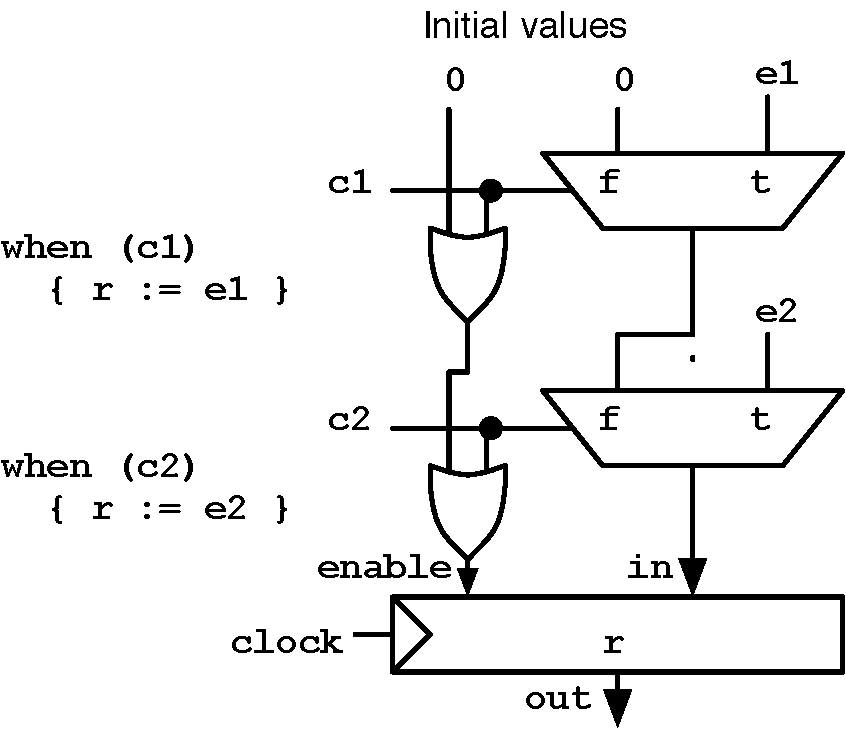
\includegraphics[height=2in]{figs/condupdates.pdf}
\end{center}

\begin{itemize}
\item Each \kode{when} statement adds another level of data mux and ORs
  the predicate into the enable chain and
\item the compiler effectively adds
  the termination values to the end of the chain automatically.
\end{itemize}

\end{frame}

\begin{frame}[fragile]{Targetting Multiple Registers}

\begin{scala}
r := Fix(3) 
s := Fix(3)
when (c1) { r := Fix(1); s := Fix(1) }
when (c2) { r := Fix(2) }
\end{scala}

leads to \kode{r} and \kode{s} being updated according to the
following truth table:

{\footnotesize
\begin{center}
\begin{tabular}{|c|c|c|c|l|}
\hline
\kode{c1} & \kode{c2}  & \kode{r} & \kode{s} & \\
\hline 
0 &  0 & 3 & 3 & \\
0 &  1 & 2 & 3 & \\ 
1 &  0 & 1 & 1 & \kode{r} updated in \kode{c2} block, \kode{s} updated using default \\
1 &  1 & 2 & 1 & \\
\hline
\end{tabular}
\end{center}
}


\end{frame}

\begin{frame}[fragile]{Conditional Update Nesting}

\begin{scala}
when (a) { when (b) { body } }
\end{scala}

which is the same as:

\begin{scala}
when (a && b) { body }
\end{scala}

\end{frame}

\begin{frame}[fragile]{Conditional Update Chaining}

\begin{scala}
when (c1) { u1 }
.elsewhen (c2) { u2 }
.otherwise { ud }
\end{scala}

which is the same as:

\begin{scala}
when (c1) { u1 }
when (!c1 && c2) { u2 }
when (!(c1 || c2)) { ud }
\end{scala}

\end{frame}

\begin{frame}[fragile]{Switch Statement}

\begin{scala}
switch(idx) {
 is(v1) { u1 }
 is(v2) { u2 }
}
\end{scala}

which is the same as:

\begin{scala}
when (idx === v1) { u1 }
.elsewhen (idx === v2) { u2 }
\end{scala}

\end{frame}

\begin{frame}[fragile]{Finite State Machines}

\begin{scala}
class Parity extends Component {
  val io = new Bundle {
    val in  = Bool(dir = INPUT)
    val out = Bool(dir = OUTPUT) }
  val s_even :: s_odd :: Nil = Enum(2){ UFix() }
  val state  = Reg(resetVal = s_even)
  when (s.in) {
    when (state === s_even) { state := s_odd  }
    .otherwise              { state := s_even }
  }
  io.out := (state === s_odd)
}
\end{scala}
\end{frame}


\begin{frame}[fragile]{Memories}

\begin{scala}
def object ROM {
  def apply[T <: Data](inits: Seq[T])(type: => T): ROM
}

def object RAM {
  def apply[T <: Data](n: Int, resetVal: T = null)(type: => T): RAM
}

class RAM[T <: Data]
    (val n: Int, val resetVal: T, val inits: Seq[T], type: () => T) 
      extends Updateable {
  def apply(addr: UFix): T
}
\end{scala}

\end{frame}

\begin{frame}[fragile]{Rom}

\begin{scala}
val i = Array(UFix(1), UFix(2), UFix(4), UFix(8))
val m = ROM(i){ UFix(width = 32) }
val r = m(counter(UFix(3)))

def sinTable (amp: Double, n: Int) = {
  val ts = Range(0, n, 1).map(i => (i*2*Pi)/(n.toDouble-1) - Pi) 
  ROM(ts.map(t => Fix(round(amp * sin(t))))){ Fix(width = 32) }
}

def sinWave (amp: Double, n: Int) = 
  sinTable(amp, n)(counter(UFix(n))
\end{scala}

\end{frame}

\begin{frame}[fragile]{Ram}

\begin{scala}
def audioRecorder(n: Int, button: Bool) = { 
  val addr   = counter(UFix(n))
  val ram    = RAM(n)
  ram(addr) := button
  ram(Mux(button, UFix(0), addr))
} 
\end{scala}

\end{frame}

\begin{frame}[fragile]{Register File}

\begin{scala}
val regs = RAM(32)
when (wr_en) {
  regs(wr_addr) := wr_data
}
val idat = regs(iaddr)
val mdat = regs(maddr)
\end{scala}

\end{frame}

\begin{frame}[fragile]{Realistic Register File}

\begin{scala}
val regfile = RAM(64){ Bits(width = 32) }
// w_mask = bit_mask
when (wen) {
  regfile(addr_in) := data_in1
}
val read_data = Reg(regfile(addr_in))
\end{scala}

\end{frame}

\begin{frame}[fragile]{Port Classes, Subclasses, and Nesting}

\begin{scala}
class SimpleLink extends Bundle { 
  val data = Bits(16, OUTPUT) 
  val rdy  = Bool(OUTPUT)
}
\end{scala}

\noindent
We can then extend \verb+SimpleLink+ by adding parity bits using
bundle inheritance:

\begin{scala}
class PLink extends SimpleLink { 
  val parity = Bits(5, OUTPUT) 
}
\end{scala}

\noindent
In general, users can organize their interfaces into hierarchies using inheritance.  

\end{frame}

\begin{frame}[fragile,shrink]{Filter Example}

From there we can define a filter interface by nesting two
\verb+PLink+s into a new \verb+FilterIO+ bundle:

\begin{scala}
class FilterIO extends Bundle { 
  val x = new PLink().flip
  val y = new PLink()
}
\end{scala}

\noindent
where \verb+flip+ recursively changes the ``gender'' of a bundle,
changing input to output and output to input.

We can now define a filter by defining a filter class extending component:

\begin{scala}
class Filter extends Component { 
  val io = new FilterIO()
  ...
}
\end{scala}

\noindent 
where the \verb+io+ field contains \verb+FilterIO+. 

\end{frame}

\begin{frame}[fragile]{Bundle Vectors}

\begin{scala}
class CrossbarIo(n: Int) extends Bundle {
  val in  = Vec(n){ new PLink().flip() }
  val sel = UFix(sizeof(n), INPUT)
  val out = Vec(n){ new PLink() }
}
\end{scala}

\noindent
where \verb+Vec+ takes a size as the first argument and a block returning a port as the second argument.

\end{frame}

\begin{frame}[fragile]{Bulk Connections}
We can now compose two filters into a filter block as follows:

\begin{scala}
class Block extends Component { 
  val io = new FilterIO()
  val f1 = new Filter()
  val f2 = new Filter()

  f1.io.x <> io.x
  f1.io.y <> f2.io.x
  f2.io.y <> io.y
}
\end{scala}

\noindent
where \verb+<>+ bulk connects interfaces.
\begin{itemize}
\item Bulk connections connect leaf ports of the same name to each other.
\item After all connections are made and the circuit is being elaborated,
Chisel warns users if ports have other than exactly one connection to them.
\end{itemize}

\end{frame}

\lstset{basicstyle={\tiny\ttfamily}}

\begin{frame}[fragile]{Port Views}
\begin{scala}
class RomIo extends Bundle {
  val isVal = Bool(INPUT)
  val raddr = UFix(32, INPUT)
  val rdata = Bits(32, OUTPUT)
}

class CpathIo extends Bundle() {
  val imem = RomIo().flip()
  val dmem = RamIo().flip()
  ...
}

class Cpu extends Component {
  val io = new CpuIo()
  val c  = new CtlPath()
  val d  = new DatPath()
  c.io.ctl  <> d.io.ctl
  c.io.dat  <> d.io.dat
  c.io.imem <> io.imem
  d.io.imem <> io.imem
  c.io.dmem <> io.dmem
  d.io.dmem <> io.dmem
  d.io.host <> io.host
}
\end{scala}
\end{frame}

\lstset{basicstyle={\footnotesize\ttfamily}}

\begin{frame}[fragile]{Bundle Vectors}
\begin{scala}
def Mux[T <: Bits](c: Bool, con: T, alt: T): T

Mux(c, UFix(10), UFix(11))
\end{scala}

\noindent
yields a \kode{UFix} wire because the \kode{con} and \kode{alt} arguments are each of type \kode{UFix}.
\end{frame}

\begin{frame}[fragile]{Bundle Vectors}

\begin{equation}
y[t] = \sum_j w_j * x_j[t-j]
\end{equation}

\begin{scala}
def innerProductFIR[T <: Num] (w: Seq[Int], x: T) = {
  val delays = Range(0, w.length).map(i => Num(w(i)) * delay(x, i))
  delays.foldRight(_ + _)
}

def delay[T <: Bits](x: T, n: Int): T =
  if (n == 0) x else Reg(delay(x, n - 1))
\end{scala}

\end{frame}

\begin{frame}[fragile]{Parameterized Classes}
\begin{scala}
class FilterIO[T <: Data]()(type: => T) extends Bundle { 
  val x = type.asInput.flip
  val y = type.asOutput
}

class Filter[T <: Data]()(type: => T) extends Component { 
  val io = (new FilterIO()){ type }
  ...
}
\end{scala}
\end{frame}

\begin{frame}[fragile]{Parameterized Classes Continued}
\begin{scala}
class ioDecoupled[T <: Data]()(data: => T) extends Bundle {
  val ready = Bool(INPUT)
  val valid = Bool(OUTPUT)
  val bits  = data.asOutput
}

class FifoIO[T <: Data]()(type: => T) extends Bundle  {
  val enq = new ioDecoupled()( type ).flip()
  val deq = new ioDecoupled()( type )
}
\end{scala}
\end{frame}


\end{document}
